\section{Research}
\subsection{Climate Change}
The consensus among scientists is that the Earth is unequivocally warming, with a high certainty that this is being caused by human activities, specifically due to the last 150 years of industrial development. The International Panel on Climate Change (\textsc{ipcc}) defines climate change as:

\begin{quote}
``A change in the state of the climate that can be identified (e.g. using statistical tests) by changes in the mean and/or the variability of its properties, and that persists for an extended period, typically decades or longer. [\ldots]any change in climate over time, whether due to natural variability or as a result of human activity''~\cite{IPCC-synthesis-07}
\end{quote}

This differs from the United Nations Framework Convention on Climate Change (\textsc{unfccc}) definition, which places the blame more squarely on human cause, where:

\begin{quote}
``[\ldots] climate change refers to a change of climate that is attributed directly or indirectly to human activity that alters the composition of the global atmosphere and that is in addition to natural climate variability observed over comparable time periods.''~\cite{IPCC-synthesis-07}
\end{quote}

There are many different responses to climate change, most focusing on either mitigation (``implementing policies to reduce \textsc{ghg} emissions and enhance sinks'')~\cite{IPCC-glossary-mitigation} or adaptation. (``Initiatives and measures to reduce the vulnerability of natural and human systems against actual or expected climate change effects. Various types of adaptation exist, e.g. anticipatory and reactive, private and public, and autonomous and planned.'')~\cite{IPCC-glossary-adaptation}

\subsubsection{United Nations Framework Convention on Climate Change}

The United Nations Framework Convention on Climate Change (\textsc{unfccc}) is an international environmental treaty which covers most of the countries in the world. It was signed in 1992 with the aim to stabilise the concentration of greenhouse gases (\textsc{ghg}) in the atmosphere ``at a level that would prevent dangerous anthropogenic (i.e. human) interference with the climate system.''~\cite{IPCC-synthesis-01-question1}

The definition of `dangerous' is up to interpretation, although the \textsc{ipcc} concluded that the definition would vary between different regions of the world, primarily dependent on the local consequences of global warming, the region's ability to adapt to climate change and the ability to reduce \textsc{ghg}. Figure~\ref{fig:burning_embers} shows the commonly named `burning embers' diagram, which represents conceptual impact across five ``reasons for concern.''

\begin{figure}[h!]
	\centering
	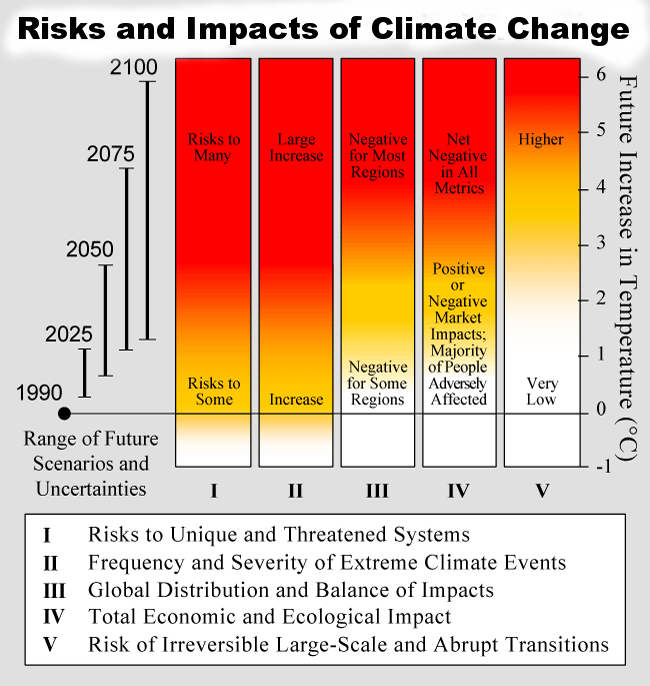
\includegraphics[width=0.6\textwidth]{img/Risks_and_Impacts_of_Global_Warming.png}
	\caption{`Burning embers' diagram~\cite{IPCC-workinggroup-01}}
	\label{fig:burning_embers}
\end{figure}

\subsection{The Kyoto Protocol}

Having recognised that developed countries are primarily responsible for the high levels of \textsc{ghg}s in the atmosphere, the \textsc{unfccc} formed the Kyoto Protocol to not only encourage countries to reduce emissions, but to commit to that reduction.~\cite{UNFCCC-kyoto-summary}To make the Protocol more appealing, carbon taxation was avoided in favour of other carbon reduction mechanisms. 

The initial agreement was signed on the 11th December 1997 during the 3rd annual \textsc{unfccc} conference and then came into force on the 16th February 2005. The Protocol sets mandatory targets on \textsc{ghg} emissions for the world's leading economies ``with a view to reducing their overall emissions of such gases by at least 5 percent below existing 1990 level in the commitment period 2008 to 2012.''~\cite[Article 2, Paragraph 1]{UNFCCC-98}. Future targets are expected to be drawn up for ``commitment periods'' after 2012.~\cite[Article 2, Paragraph 4]{UNFCCC-98}

As of September 2011, 191 countries have ratified the treaty with the United States remaining as the only signatory not to have ratified the protocol. However, some United Nation member states such as Afghanistan, Andorra, and South Sudan never signed the agreement and Canada left in December 2011.

The aim of the Kyoto Protocol is to contain emissions of anthropogenic \textsc{ghg}s in a way that reflects underlying national differences in emissions, wealth, and capacity for reduction; this concept is known as ``common but differentiated responsibilities.''~\cite{Grubb-04}\cite{UNFCCC-92} It was recognised that much of the existing \CO emissions were due to developed countries, and that the needs of developing countries would need to be taken into account when calculating emission targets. It was agreed that the per capita emissions of developing countries was still relatively low, and that these participants would be allowed to grow to meet their socio-economic needs.

Participants in the Kyoto Protocol were classified into three groups, according to their responsibilities:~\cite{UNFCCC-92}

\begin{description}
	\item[Annex I] \hfill \\
	Industrialised countries and economies in transition. These countries have committed to reduce their emissions levels of greenhouse gases to targets that are set according to their 1990 emissions.
	
	\item[Annex II] \hfill \\
	Developed countries. Annex II countries are a subset of Annex I countries, and are encouraged to invest in developing countries.

	\item[Non-Annex] \hfill \\
	Developing countries which are not required to reduce emission levels unless developed countries have supplied funding and technology through outsourcing. This serves three purposes:
	\begin{itemize}
		\item To avoid restricting a country's development, since burgeoning economies tend to rely on carbon based industry.
		\item To permit sale of excess emission capacity to those nations having difficulty meeting their targets.
		\item To encourage investment from Annex I countries in low-carbon technology.
	\end{itemize}
\end{description}

The Protocol structures rolling emission reduction commitment periods, with the first scheduled to end in 2012.

\subsubsection{Initial Commitment Period}

Parties partaking in the Kyoto Protocol commit themselves to reducing four \textsc{ghg}s (carbon dioxide, methane, nitrous oxide, and sulphur hexafluoride) and two other groups of gases (hydrofluorocarbons and perfluorocarbons). These are considered \CO equivalents when calculating emission reduction.

With the understanding that only Annex I countries have targets that they must commit to, the aim is to reduce global \CO emissions to at least 5\% below the base year by the end of the first commitment period. Through negotiation, the base year decided on was 1990, due to the lack of accurate data for years prior to this. Participants would need to agree to their individual targets in line with the global target, the results of which can be read in Annex B of the Convention\cite{UNFCCC-98}. It should be noted that the \textsc{eu}-15 opted for a `burden sharing agreement' whereby the \textsc{eu} set a target of -8\%, and assigned individual targets to its member states.

Countries can meet their targets by reducing their greenhouse gas output or by offsetting their output by using the flexible mechanisms outlined in the Protocol. Even if Annex I countries meet their targets for the first period, future reductions will be required if the overall goal of \textsc{ghg} stabilisation is to become a reality.

\subsubsection{Flexible Mechanisms}

While participant countries must meet their emission targets primarily through domestic carbon reduction methods, Flexible Mechanisms were also put in place to make targets more attainable and affordable. These market based mechanisms help stimulate sustainable development through technology transfer, help countries with Kyoto commitments to meet their targets in a cost-effective way, and encourage the private sector and developing countries to contribute to emissions reduction. The three mechanisms defined in the Protocol are:

\begin{description}
	\item[Emissions Trading] \hfill \\
	Member states can trade a newly created commodity representing the surplus created if their emissions are below their assigned target.
	
	\item[Clean Development Mechanisms] \hfill \\
	Annex I \& II countries can invest in sustainable, greenhouse gas reduction projects in Non-Annex countries in exchange for `Certified Emission Reductions' (\textsc{cer}).~\cite{UNFCCC-05}

	\item[Joint Implementation] \hfill \\
	Annex I countries can invest in sustainable greenhouse gas reduction projects in other Annex I countries as an alternative to national reduction.
\end{description}

\paragraph{International Emissions Trading}

With international markets already trading in commodities, Article 17 of the Protocol allows for countries to sell their excess `Assigned Amount Units' (\textsc{aau}s) to countries unable to meet their target. This ability for countries to sell their excess capacity saw the birth of the `carbon market'.

Some Annex I countries, categorised as Economies In Transition (\textsc{eit}), have a large surplus of \textsc{aau}s, which can be sold on the carbon market. One example is Russia: having closed many cold-war-era industries since its 1990 base year, Russia was given more headroom for growth when its carbon target was set. Despite the abundance of \textsc{aau}s in the market, to stop countries overselling units and becoming unable to meet their own targets, participants must keep a reserve of \textsc{aau}s (known as a `commitment period reserve') which cannot fall below 90\% of its assigned amount.

\subparagraph{European Union Emission Trading System}

The European Union Emission Trading System (\textsc{eu ets}) allows for trading between participants in the EU and between industry operators in the \textsc{eu}. Governments of \textsc{eu} states agree on national emissions caps, and then allocate allowances to their industrial operators. Operators may privately move allowances between themselves, privately match buyers and sellers, or trade on the carbon exchange. Trading has proved to be very unpopular outside of the \textsc{eu}.~\cite{Grubb-09}

\paragraph{Clean Development Mechanisms}

Article 12 of the Protocol allows for Clean Development Mechanisms (\textsc{cdm}), whereby Annex I countries may invest in emission-reducing projects in developing countries. In exchange, projects earn saleable \textsc{cer} credits, which the investor may use to meet their target. Article 12 of the Protocol describes its objectives:

\begin{itemize}
	\item Assist Annex I parties to develop sustainable emission-reduction projects in Non-Annex countries (in line with the primary \textsc{unfccc} goal).
	\item Assist Annex I parties to meet their emission targets.
\end{itemize}

Figure~\ref{fig:cdm_map} shows a map of \textsc{cdm} projects worldwide.

\begin{figure}[h!]
	\centering
	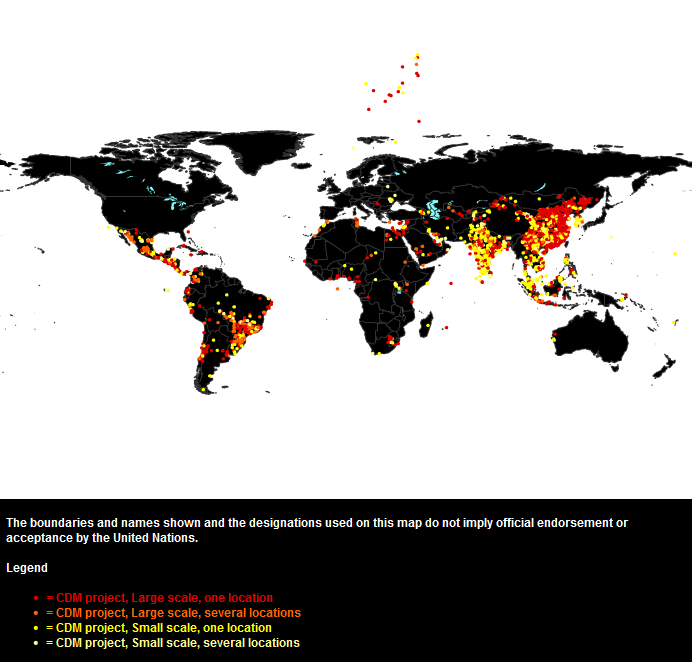
\includegraphics[width=0.8\textwidth]{img/CDM_Map.png}
	\caption{Map of \textsc{cdm} projects worldwide~\cite{UNFCCC-CDM-map}}
	\label{fig:cdm_map}
\end{figure}

Industrialised countries wishing to take part in \textsc{cdm} need to get assurance from the project host that it will contribute to sustainable development. The applicant must also prove that the project would not have happened regardless of their support, and must project future emissions had the project not gone forward. This ensured there are no `free riders' and that the applicant is awarded the correct amount of units for their contribution to the project.

\paragraph{Joint Implementation}

Article 6 defines the Joint Implementation (\textsc{ji}) mechanism, which allows countries to invest in carbon-reduction projects in other Annex I countries as an alternative to national emission reduction. In exchange for the investment, the investor will be awarded an Emission Reduction Unit (\textsc{eru}), which is to be taken from the investee's \textsc{aau} pool. This requirement ensures that the total amount of units shared between Annex I countries does not change during a commitment period.

\textsc{ji} may be advantageous where carbon reduction is cheaper to implement in another Annex I country rather than nationally (an example might involve replacing dirty power plants with cleaner energy producers). To date, \textsc{ji} has not been very popular, with only 22 projects having been registered prior to 2008. %citation needed

\subsubsection{Reporting, Monitoring, and Sanctioning}

Each participant must designate an authority to create and manage its \textsc{ghg} inventory. While not specifically required, many Non-Annex countries have also set up national bodies to manage their Kyoto obligations (primarily \textsc{cdm}s).

Kyoto requires that:~\cite{UNFCCC-Kyoto-guidelines}

\begin{itemize}
	\item Annex I countries must have in place a national system to estimate \textsc{ghg} emissions (natural and anthropogenic) and any \CO that has been removed through sinks.
	\item Annex I countries must report their greenhouse inventories annually and provide regular communication detailing supplementary information to demonstrate compliance.
	\item Expert review teams periodically review greenhouse inventories and any national communications (this must be conducted at least once every 5 years).
\end{itemize}

The efficacy of the Kyoto Protocol depends on the participants following the Protocol's rules and regulations with respect to their commitments and the accuracy and reliability of their reports. Keeping in line with the core aim of the Kyoto Protocol (that is, an alternative to a carbon tax) financial sanctions were avoided, instead opting for the setting of harsher emissions targets.

Part of monitoring involves an expert review of reports submitted by participants. Reviewers may mark reports as `question of implementation' where there is an unresolved problem regarding implementation, may suggest `adjustment' where inventory is incomplete, and may suggest `correction' where there are clear inconsistencies (suggesting `cheating'). `Correction' is analogous to an inventory adjustment.~\cite{UNFCCC-reporting-review}

There are also sanctions for parties not meeting the emissions target they committed to. If the enforcement branch determines that Annex I countries do not comply with their emissions limitations, that country is required to make up the difference in future commitment periods plus an additional 30\%. That country will also be suspended from emissions trading.~\cite{UNFCCC-compliance}

\subsubsection{Criticisms}

Opinions on the effectiveness of the Kyoto Protocol vary significantly; while some consider it a move in the right direction for the stabilisation of \textsc{ghg} emissions, others believe the Protocol is inherently unfair and ineffective.

\paragraph{Inception}
Problems of fairness were raised early in the negotiation stages of the Protocol. During the negotiations for the setting of the base year, 1990 was chosen as reliable data prior to this date was unavailable. This base year was also highly favoured by the \textsc{uk}, Germany, and Russia as their respective \CO levels were high in 1990. Following 1990, \textsc{uk} emissions dropped as the energy sector moved away from coal power, toward cleaner gas power stations. Germany's \CO emissions also decreased following 1990 when East Germany and West Germany reunited, resulting in a decrease in dirty industry in East German territories. There was much disagreement as Japan wished to use 1995 as the base year, while former Soviet block countries wanted to use emission rates from before their industrial collapse at the end of the cold war.

There were also disagreements over the size of the emission cuts, with the \textsc{eu} supporting cuts in the range of 10-15\%, while the \textsc{us} wanted a more conservative cut of between 0-5\%. The level of cutbacks wanted varied from country to country, with the only common theme being that the proposals suited the interests of the country making the proposal.~\cite{Grubb-economics}

\paragraph{Trading}
There was also concern regarding the implementation of emissions trading. The \textsc{eu} and Japan wanted to ensure that emission trading was free and transparent, and wanted to prevent the \textsc{us} from using its political pressure to gain preference when trading with Russia. This concern was echoed in developing countries, where they believed the \textsc{us} would use flexibility mechanisms to its own advantage, over the interests of less able countries that needed support.

With Russia having an abundance of \textsc{aau}s, there was concern that it would have a monopoly on the carbon trading market, and would be able to adversely affect the price of carbon. Russia could withhold \textsc{aau}s to inflate the price for units, and inflate its profits. While possible, the situation was also difficult for Russia, since it has both an excess of \textsc{aau}s, and was one of the largest oil producers. Selling \textsc{aau}s would encourage the purchasing of oil, while withholding \textsc{aau}s would increase their value, but might adversely affect the price of fossil fuels.

\paragraph{The effect of Non-Annex countries}

Following successful negotiation and signing of the Protocol, concern was raised regarding the lack of limitations on the \textsc{ghg} emissions of developing countries. Indeed the \textsc{us} did not ratify the Protocol, stating that ``it exempts 80\% of the world, including major population centers such as China and India, from compliance, and would cause serious harm to the \textsc{us} economy''.~\cite{Hague-to-Marrakesh} Statistics from the International Energy Agency (\textsc{iea}) show by 2011, emissions from Non-Annex countries had exceeded those from Annex I countries.~\cite{IEA-highlights} Only 3 countries from the top 10 table of carbon emitters are currently an Annex I participants.

\subsection{Common Pool Resources}

A Common Pool Resource (\textsc{cpr}) is a natural or man-made resource in which: the resource is deductible; the size and characteristic of the resource make it difficult to exclude other from its use.~\cite{Ostrom-90} \textsc{cpr}s are defined by their core resource (\emph{stock variable}) and the limited quantity of extractable units (\emph{flow variable}). The stock variable is to be conserved such that consumers may continue to exploit/consume excess resources (\emph{fringe variable}), which are produced at a rate defined by the flow variable.

Due to a \textsc{cpr}'s deductible, non-exclusive characteristics; it may suffer from congestion or overuse. Many \textsc{cpr} systems form positive feedback loops, and so with careful resource management (ensuring the stock variable is not compromised), fringe units will be continually produced, allowing for efficient operation. Excessive consumption (consumption exceeding the flow variable) will reduce the stock variable, which in turn will reduce the flow variable. Unless the stock variable is allowed to regenerate, excessive use will result in resource depletion; even if the stock is allowed to regenerate, the damage may be irreparable. The key to efficient \textsc{cpr} is to ensure the resource is not abused.

An example of \textsc{cpr} is commercial fishing; by overfishing certain species of fish, the stock variable (number of fish) is reduced, which in turn reduces the flow variable (birth rate), which decreases the fringe units which can be sustainably caught by fishers. Unless the stock variable is allowed to regenerate, certain species of fish may be driven to depletion (extinction). This is an example of inefficient use of a \textsc{cpr}, the only viable solution to which is drastically reducing the rate of fishing. This, and further example cases, are discussed in more detail later.

While some \textsc{cpr}s are owned by governments or private parties, making these public or private goods, many have no ownership, and so are an open access resource. We should note the difference between `Common Pool Resources', as described above, and `The Commons', which

\begin{quote}
	``refer to systems, such as knowledge and the digital world, in which it is difficult to limit access, but one person's use does not subtract a finite quantity from another's use.''~\cite{Ostrom-challenge-90}
\end{quote}

With the understanding that uncontrolled access to a \textsc{cpr} will lead to inefficiencies and overuse, some resource consumers form an institution, often called a `Common Property Regime', to reduce the threat to the common resource by independent actions and increase the efficiency of resource harvesting.

\subsubsection{Common Property Regime}

Common Property Regimes are formed to protect and maintain resource systems by coordinating strategy. These strategies are based on the protection of the core resource, with fringe units being allocated to participants based on an arranged scheme. While regimes can be effective at protecting \textsc{cpr}s, the difficulty is in the devising of rules, limits, sanctions, and other operational variables.

The correct setting of appropriation limits is important, as setting limits too low could lead to overuse and eventual depletion of the resource, conversely setting limits too high reduces the efficiency at which the resources can be harvested. In Common Property Regimes, access to the common property is no longer free; those outside the regime see the resource as a private good, while those part of the regime see it as common good (albeit one in which appropriation is carefully monitored.)

Elinor Ostrom defined eight design principles which are required for an effective Common Property Regime:~\cite{Ostrom-90}

\begin{itemize}
	\item Clearly defined boundaries
	\item Congruence between appropriation and provision rules and local conditions
	\item Collective choice arrangements allowing for the participation of most of the appropriators in the decision making process
	\item Effective monitoring by monitors who are part of or accountable to the appropriators
	\item Graduated sanctions for appropriators who do not respect community rules
	\item Conflict-resolution mechanisms which are cheap and easy of access
	\item Minimal recognition of rights to organize (e.g. by the government)
	\item In case of larger \textsc{cpr}s: Organisation in the form of multiple layers of nested enterprises, with small, local \textsc{cpr}s at their bases
\end{itemize}

Indeed Ostrom continues to say:

\begin{quote}
	``When subjects are placed in settings in which decisions are made in isolation, with minimal institutional structure, their aggregate behaviour is generally consistent with equilibrium predictions of inefficient resource use. On the other hand, when allowed to communicate or use other coordinating mechanisms, subjects often adopt and maintain agreements consistent with efficient and sustainable resource use''~\cite{Ostrom-rules}
\end{quote}

\subsubsection{Case Study}

These case studies look at examples of \textsc{cpr}s in the real world, the strategy behind these, and whether theses are considered a success.

\paragraph{Commercial fishing}

In the 70s, the fishing industry was in danger of shrinking due to overfishing. The measures taken to prevent this are analogous to that of a CPR problem. This makes it a good example to demonstrate the theory of \textsc{cpr}.

In 1979 the \textsc{un} set out new regulations and `protected zones' for each country with a coastline.~\cite{Canada-sea-law} \textsc{cpr} models suggest that when individuals are allowed to make decisions in isolation, with minimal institutional structure, the aggregate behaviour will be inefficient. In other words, left to their own devices each countries' fishermen would take as many fish as possible, leading to the eventual depletion of the resource. By putting institutional rules in place, the \textsc{un} were aiming to control the behaviour of the individuals (fishermen).

``[\ldots]not only do governments now have the legal power and the self-interest to apply sound principles of resource management within this area, but they have an obligation to do so.''

The aim of the new regulations was to get all the countries to cut back their fishing by an equal proportion, which is exactly how a typical \textsc{cpr} problem is solved. However, instead of imposing restrictions on fishing, many countries expanded their fishing fleets to take advantage of their new `property'. This was due to incorrect data and models used by various countries when calculating what limitations would need to be put in place, which indicated an increase was feasible.

\paragraph{Ozone Layer \& CFCs}

Scientists in the 1970s discovered an area of the Antarctic stratosphere with very low levels of ozone (33\% less than ozone level for that area pre-1975), which became known as the ozone hole. The increasing ozone layer depletion would eventually led to significantly more \textsc{uv} radiation reaching the surface of the Earth, with possibly disastrous effects.

Chlorofluorocarbons (\textsc{cfc}s) were to blame for this destruction of the ozone layer, with a single \textsc{cfc} molecule having the power to chemically unbind 4000 molecules of the ozone. The individuals in this case were the manufacturers working with \textsc{cfc}s. Their isolated decisions would be to not regulate their \textsc{cfc} usage at all, in order to maximize the profit made on their products. Consequently, the ozone layer was in danger of being totally completed.

A regime was put in place, the `Montreal Protocol on Substances that Deplete the Ozone Layer', which set out plans to cut production of \textsc{cfc}s by 100\% over 10 years. The benefit provided by the ozone layer outweighed the increased cost to manufacturers and consumers caused by the removal of \textsc{cfc}s from industrial manufacturing processes. This reflects CPR theory, where by applying institutionalised proportional cutbacks, a shared resource can be used sustainably.

The ozone holes have now ceased growing (and will eventually disappear), and so this example case of \textsc{cpr} can be considered a success.

\paragraph{Analysis}

The success of schemes to protect \textsc{cpr}s worldwide varies substantially. The key to success is understanding that there is no `one-size-fits-all' solution to the problem of common resources, and that often quick fixes can cause more harm than good. While Ostrom's design principles are an integral part of Common Property Regimes, studies on the relative successes of \textsc{cpr} implementation has shown that there are a few requirements for a successful regime:~\cite{Ostrom-challenge-90}

\begin{description}
	\item[Achieving accurate and relevant information] \hfill \\
	Published information must combine accurate scientific data with an understanding of the environmental system. With the continually evolving environment, data must be kept up to date so that it is relevant. 
	
	\item[Dealing with conflict] \hfill \\
	When resources are allocated, conflict over policy and administration of regime will certainly occur. Conflicts should not be ignored, but dealt with immediately to ensure these do not become a problem further down the line. 

	\item[Enhancing rule compliance] \hfill \\
	Rules are only effective when participants consider these legitimate, fair and enforced. Participants should take some responsibility for monitoring.
	
	\item[Providing infrastructure] \hfill \\
	Physical, technological, and institutional infrastructures must be provided such that participants may operate effectively within the regime
	
	\item[Encourage adaptation and change] \hfill \\
	It is difficult to `fix' institutions for the long term, when they are still dealing with past issues. Institutions must embrace changes as part of their developments.
\end{description}

\subsubsection{The Kyoto Protocol as a CPR}

The problem which the Kyoto Protocol attempts to resolve, the reduction and stabilisation of global carbon emissions, is not dissimilar to other \textsc{cpr} problems already discussed in this report. Both the Kyoto Protocol and \textsc{cfc} reductions are \text{cpr} systems which have a global effect on the environment, economies, and development. The difference between these problems however, is one of scale.

In the first instance, Kyoto is an open resource with no real ownership; this makes it difficult to impose regulations and limitations on emissions, even if a Common Property Regime is formed. Unlike the \textsc{cpr} system involving fisheries, dividing up the world’s atmosphere by country does not prevent the actions of other adversely affecting the global environment, and unlike the problem of \textsc{cfc}s, the economic consequences are large and affect the development of countries, not just individual industries.

As in the overfishing example, participants will always attempt to play to their advantage. We have seen this to be the case in Kyoto, as described in the Criticisms subsection of the report, and this may lead to inefficiencies within the Kyoto \textsc{cpr} system. While the long term gains from participating in the Protocol are obvious, some have more to gain than others, particularly in the short term. Russia, with its excess of \textsc{aau}s has the potential to make money on the emissions trading system (or indeed, play with the market to increase profits).

The \textsc{eu}, having seen the efficiency advantages of working as part of a common regime, have further imposed regulations, systems, and sanctions within the member states. The aim of this is to ensure \textsc{eu} members are as efficient as possible within the scope of the \textsc{cpr}. Indeed this appears to be the case, as most \textsc{eu} states are on track to meet their target.~\cite{EEA-Tracking-progress-20}

Research has also shown that there may be problems of efficiency when there are significant wealth and technology inequalities. Where there are no regulations for a \textsc{cpr}, technology inequalities can exacerbate inefficient use and those participants with better technologies over-extract from the core resource, while less technologically advanced participants will lag behind. Where \textsc{cpr}s are regulated, efficiency gains from  the regime will be lower as inequality amongst participants increases. This has somewhat been avoided in the Kyoto Protocol by the introduction of Clean Development Mechanisms; this allows Annex I countries to invest in clean development in Non-Annex countries, thereby reducing the technology gap between developing and developed countries, which in turn increases the efficiency of participants in this regime.~\cite{Wealth-inequality-regulated}\cite{Wealth-inequality-unregulated}

\paragraph{Summary} It appears that Kyoto can be mapped to a Common Pool Resource scheme, and while some of the problems faced by other \textsc{cpr} systems have been carefully thought out (efficiency of regimes, \textsc{cdm} to combat wealth inequality), other problems still remain (no limits for Non-Annex countries, countries playing Kyoto to their advantage), which may cause long term problems to the efficacy of the protocol.

\subsection{Multi-Agent Systems}

\subsubsection{Definition}

A multi-agent system (\textsc{mas}) is a paradigm for conceptualising, designing, and implementing a system composed of multiple intelligent agents within an environment. We can therefore use \textsc{mas} as a model to portray computing as a process of interaction~\cite{MAS-DoC} where agents can autonomously cooperate, reach agreements, or even compete with other agents that have different interests.  Thus topics such as portfolio management~\cite{Warren-ISA}, joint mission planning,~\cite{Joccasta-ISA} and the modelling of social structure~\cite{jasss-soc-surrey} are areas where \textsc{mas} research may be an appropriate approach.

A \textsc{mas} has the following advantages over a single agent or centralised approach:

\begin{itemize}
	\item A \textsc{mas} distributes computational resources and capabilities across a network of interconnected agents. In addition, a \textsc{mas} should not suffer from resource limitations, performance bottlenecks, and/or critical failures due to its decentralised nature.

	\item A \textsc{mas} allows for agent wrappers around one or more existing legacy systems which allows them to be incorporated into an agent society.

	\item A \textsc{mas} efficiently retrieves, filters, and globally coordinates information from sources that are spatially distributed.

	\item A \textsc{mas} provides solutions in situations where expertise is spatially and temporally distributed.
\end{itemize}

\subsubsection{Structure of an Agent}

Agents are very similar to active concurrent objects except for one key difference: agents can decline to perform an action (e.g. refusing a trade proposition in a trading simulation). Often, they also interact using a common high level peer to peer (\textsc{p2p}) communication language, which allows them to coordinate their activities asynchronously. These similarities do mean that concurrent object oriented programming is a suitable base for building multi agents systems.

As mentioned previously, \textsc{mas} are composed of agents and an environment as seen in Figure~\ref{fig:mas}. Therefore it is essential that agents are able to perceive the environment where they are situated (e.g.: via sensors, message reception, or event detection) giving partial information on its state and that they are also able to act upon it with possible non-deterministic outcomes (e.g.: via effectors).

\begin{figure}[h!]
	\centering
	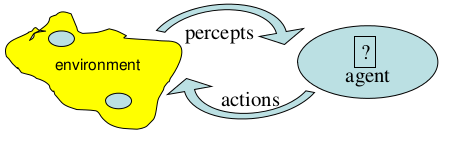
\includegraphics[width=0.6\textwidth]{img/mas.png}
	\caption{Basic multi agent system structure}
	\label{fig:mas}
\end{figure}

This allows the programmer to design proactive agents, which are set out to achieve ``well defined goals''. Agents' behaviours are thus goal directed. This requires the environment to be maintained in a certain state and the agent to achieve a certain state of its environment.~\cite{MAS-DoC}

From a software engineering perspective, the most adapted agent structure for our project is to use agents with states as shown in Figure~\ref{fig:agent-architecture}.

\begin{figure}[h!]
	\centering
	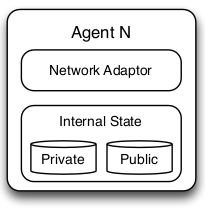
\includegraphics[]{img/agent-architecture.png}
	\caption{General agent architecture~\cite{Sam-Transfer-Report}}
	\label{fig:agent-architecture}
\end{figure}

We can use the agent's internal data to record information about the environment state and its history. Separating the internal state into public and private sectors also allows the agent to keep some information hidden from other querying agents. Finally, all \textsc{p2p} messages are sent via a network adapter which allows us to abstract away communication protocols and methods.

\subsubsection{Services and Protocols}

In order to simplify the implementation of agents, it was agreed that we would require additional services and protocols on top of the environment and network. Services allow us to retrieve the environment shared state raw data in a more user-friendly way. Similarly, protocols encapsulate inter-agent communication.

By using such components, we can encase the software implementation of our simulation framework. Any changes made to the way the environment stores data or how communications are handled would therefore not affect the behaviour of our agents.

\subsubsection{Presage2}

There exist several platforms that allow the development of multi agent systems. The two most important ones are Jade and Repast. However, it was decided to use the internally developed Presage 2 platform due to the nature of our desired simulation.

Originally written by Brendan Neville and then improved by Sam MacBeth, the platform offers the ability to rapidly prototype complex agent societies. In Presage 2, agents are allowed to act during incrementing time steps, which results in discrete time driven simulations. It also offers a rich communication layer as well as the ability to batch multiple simulation runs through a web user interface. Finally, the following requirements are met, which allow for the design of social behaviour and the observation of long term global performance and adaptation~\cite{Presage2-agent-societies}:

\begin{description}
	\item[Abstraction:] the agents and network can be as simple or complex as necessary (e.g.: agents can range from being simply reactive to implementing complex belief, desire and intentions (BDI).)

	\item[Flexibility:] the platform allows the user to easily change the simulation input parameters. In conjunction with the ability to batch run, it is very simple to measure the impact of variable values.

	\item[Extensibility:] base classes and modules can be extended in order to allow the user to add any desired functionality.

	\item[Interaction:] Simulation data can be stored in a MongoDB collection which provides easy access and visualisation of the results.

	\item[Rule engine:] There is support for executable, mutable rule specifications.
\end{description}

Figure~\ref{fig:presage2-architecture} and \ref{fig:presage2-lifecycle} respectively show Presage 2's general architecture and the breakdown of a simulation run:

\begin{figure}[h!]
	\centering
	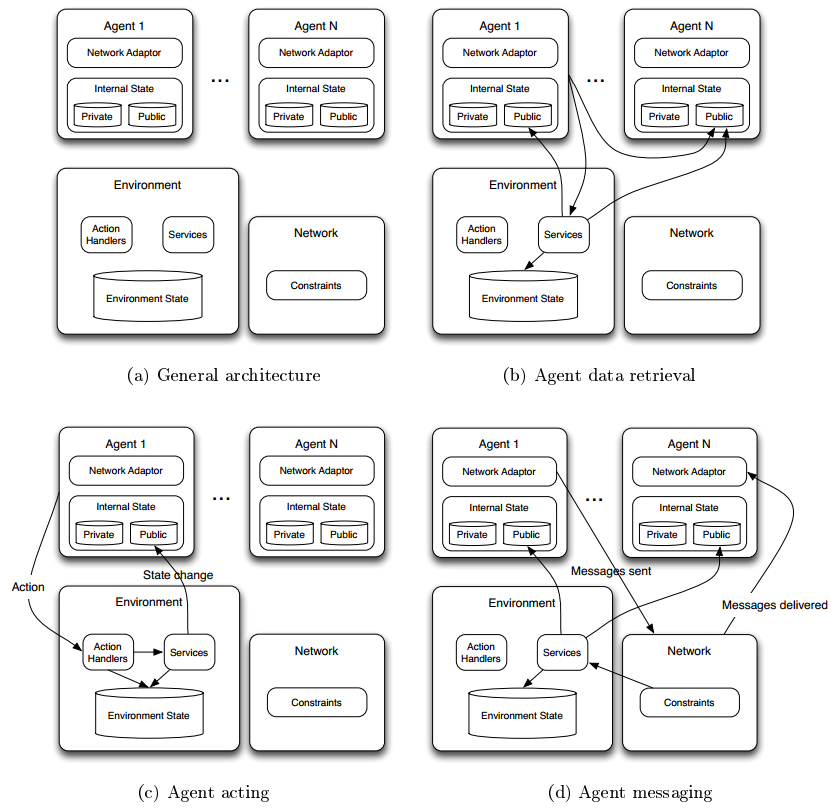
\includegraphics[width=\textwidth]{img/presage2-arch.png}
	\caption{Presage2 architecture~\cite{Sam-Transfer-Report}}
	\label{fig:presage2-architecture}
\end{figure}

\begin{figure}[h!]
	\centering
	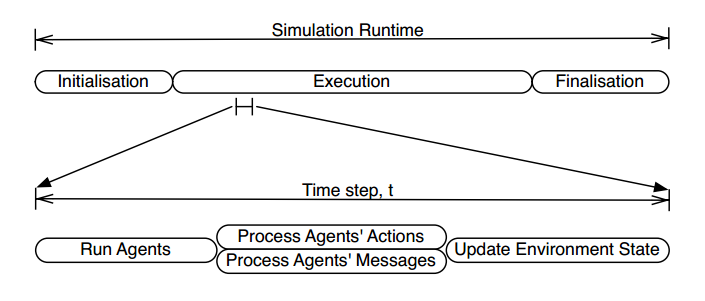
\includegraphics[width=\textwidth]{img/presage2-lifecycle.png}
	\caption{Presage2 simulation architecture~\cite{Sam-Transfer-Report}}
	\label{fig:presage2-lifecycle}
\end{figure}
